\chapter{The Evolution of Cheating: From Debugging Tools to an Organized Industry}

The history of cheating in video games is deeply intertwined with the evolution of the industry itself. What began as debugging tools for developers gradually transformed into a clandestine culture of modifications, and with the advent of online gaming, an organized and profitable industry with ties to cybercrime \parencite{consalvo2007cheating}. Simultaneously, the fight against cheating led to the development of \textbf{anti-cheat systems}, which evolved from simple integrity checks to sophisticated solutions incorporating artificial intelligence and deep system access \parencite{yan2005cheats}.

\section{The Early Days: Debugging Tools and Experimental Modifications}

Before video games became a mainstream form of entertainment, early cheating emerged as a necessity within software development. In the 1970s and 1980s, developers embedded debugging tools within their games to facilitate testing. These systems allowed programmers to modify internal values such as lives, ammunition, and speed, enabling them to test different scenarios without playing through the entire game \parencite{smith2018konami}.

Some of these tools remained accessible in commercial releases, either unintentionally or as a deliberate choice by developers. This led to the creation of the first \textbf{cheat codes}, which were key combinations or commands that altered gameplay. One of the most iconic examples is the \textbf{Konami Code} (↑ ↑ ↓ ↓ ← → ← → B A), introduced in \textit{Gradius} (1986) and later popularized in \textit{Contra} (1988) \parencite{kent2001ultimate}. While these codes were not designed to affect competition, they set a precedent for the intentional modification of gameplay.

\section{The Rise of Cheating in Consoles and PC}

As the video game industry grew throughout the 1980s and 1990s, cheating expanded beyond debugging tools and built-in cheat codes. With the advent of home consoles, external devices specifically designed to modify gameplay began to appear.

\subsection{Cheat Devices: Game Genie, GameShark, and Pro Action Replay}

The first dedicated cheat devices were \textbf{modification cartridges}, such as the \textbf{Game Genie} (1990) and the \textbf{GameShark} (1995). These hardware add-ons allowed players to inject custom modifications into a game’s memory, altering key parameters such as health, ammunition, and physics \parencite{supercade2001}. While initially marketed as harmless tools for enhancing single-player experiences, they introduced the concept of \textbf{real-time game manipulation}, which would later be adapted for online environments.

On the PC side, the introduction of \textbf{memory editors} provided users with a more flexible and powerful way to modify game values at runtime. Early programs like \textbf{Cheat Engine} (2000) enabled players to search for specific in-game variables and alter them directly, bypassing the limitations of built-in cheat codes \parencite{gamersatwork2012}. This shift from \textbf{developer-sanctioned cheats} to \textbf{unauthorized external modifications} laid the foundation for more advanced game-hacking techniques.

As gaming technology evolved, so did the tools available for modifying game memory structures. More sophisticated programs such as \textbf{ReClass.NET} emerged, allowing users to analyze and modify game memory at a structural level. Unlike traditional memory scanners, ReClass.NET enables users to reverse-engineer game memory layouts by dynamically inspecting class structures and data offsets in real-time \parencite{wang2015reclass}. This advancement significantly improved the ability of cheat developers to create complex modifications, from automatic aimbots to more intricate exploits that manipulate how game logic processes data.



\begin{figure}[h!]
    \centering
    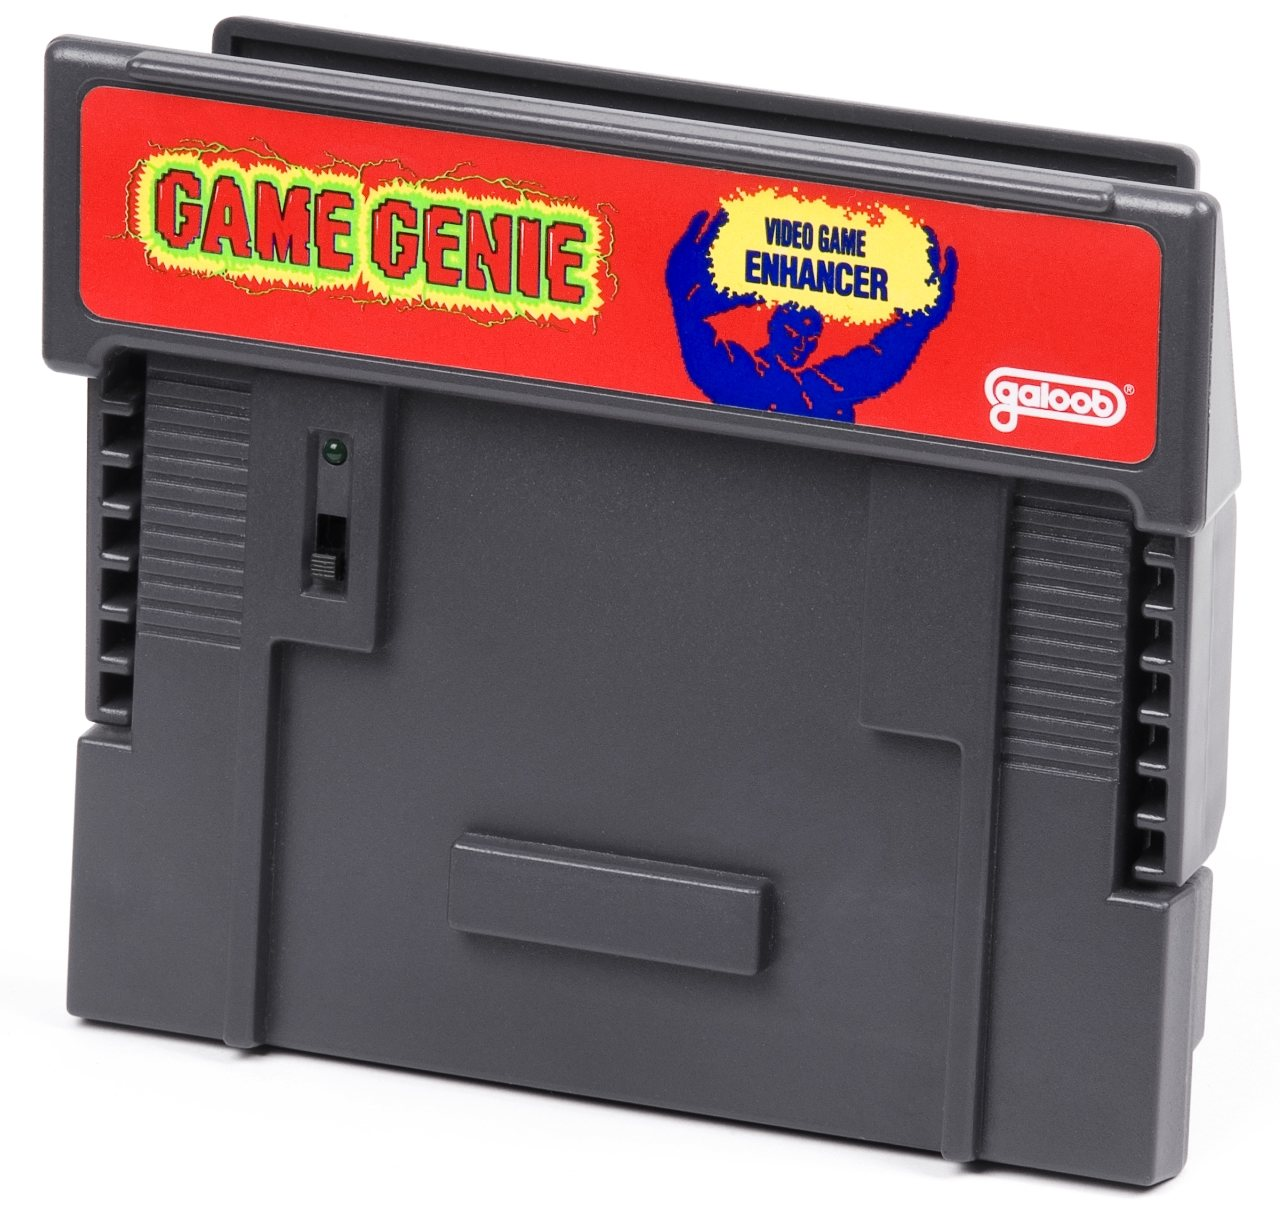
\includegraphics[width=0.5\linewidth]{images/logo-12.jpg}
    \caption{Game Genie}
    \label{fig:enter-label}
\end{figure}

\newpage
These tools, originally designed for educational and debugging purposes, soon became widely used in cheat development, particularly in online gaming environments. Their increasing complexity meant that anti-cheat systems had to adapt rapidly, leading to an ongoing technological arms race between cheat developers and security teams.

\section{The Transition to Online Gaming: Cheating Becomes a Competitive Threat}

The rise of online multiplayer gaming in the late 1990s and early 2000s fundamentally changed the impact of cheating. Unlike single-player cheats, which only affected the individual experience, \textbf{online cheating directly disrupted fair competition} \parencite{yan2005cheats}. As games like \textbf{Quake} (1996), \textbf{Counter-Strike} (1999), and \textbf{Diablo II} (2000) introduced matchmaking and ranking systems, the incentive to cheat increased dramatically \parencite{young2016history}.

The growing importance of competitive integrity led developers to take more aggressive measures against cheating, resulting in the creation of \textbf{server-side and client-side anti-cheat mechanisms}. However, as anti-cheat solutions became more sophisticated, so too did cheating techniques, leading to an ongoing technological arms race between game security teams and cheat developers.


This shift led to the development of the first organized cheat communities, where players and programmers shared exploits, scripts, and modified game clients. It also marked the beginning of an \textbf{arms race} between cheat developers and game security teams, as new forms of cheating emerged alongside increasingly complex anti-cheat measures.

\section{The Birth and Evolution of Anti-Cheat Systems}

As online gaming became increasingly competitive, the integrity of fair play was challenged by the widespread use of cheats. Unlike single-player modifications, which had no broader consequences, cheating in multiplayer environments compromised \textbf{matchmaking, rankings, and esports competitions}, creating frustration among players and damaging the credibility of competitive gaming. 

Early attempts to mitigate cheating relied on \textbf{server-side validation}, where game servers monitored player actions for anomalies that suggested external manipulation. These checks aimed to detect unnatural behavior, such as \textbf{impossible movement speeds, improbable accuracy, and modifications to game assets} that altered visibility constraints. However, this approach had significant limitations, as many cheats operated entirely on the \textbf{client side}, modifying game data before it was transmitted to the server. As a result, more sophisticated \textbf{client-side anti-cheat solutions} were developed to monitor and detect unauthorized modifications directly within the player’s system.

One of the first dedicated anti-cheat programs was \textbf{PunkBuster}, developed by Even Balance, Inc. and introduced in \textbf{2000}. Initially implemented in \textit{Return to Castle Wolfenstein} and later in \textit{Battlefield 1942}, PunkBuster marked a shift from basic server-side detection to \textbf{active client-side monitoring}. It worked by scanning a player’s system for \textbf{known cheat signatures}, verifying \textbf{game file integrity}, and capturing periodic \textbf{in-game screenshots} to identify visual modifications such as \textbf{wallhacks}. Additionally, PunkBuster maintained a \textbf{global ban list}, preventing known cheaters from accessing protected servers. Despite these advancements, \textbf{cheat developers quickly adapted} by employing techniques such as \textbf{code obfuscation}, allowing their software to remain undetected. PunkBuster also faced criticism for its \textbf{aggressive scanning approach}, which occasionally resulted in \textbf{false positives}, banning legitimate players due to conflicts with background applications.

In \textbf{2002}, Valve introduced \textbf{Valve Anti-Cheat (VAC)} alongside \textit{Counter-Strike 1.6}, implementing a more \textbf{automated and data-driven approach} to cheat detection. Unlike PunkBuster, which \textbf{immediately expelled} suspected cheaters, VAC introduced a \textbf{delayed banning system}. This strategy allowed suspected cheaters to continue playing while logging their infractions, making it harder for cheat developers to \textbf{identify detection triggers} and modify their cheats accordingly. In addition to \textbf{signature-based detection}, VAC utilized \textbf{heuristic analysis} to recognize \textbf{abnormal behavioral patterns}, refining its detection algorithms over time. By integrating \textbf{server-side validation} with \textbf{machine learning techniques}, VAC continuously improved its ability to detect and counteract evolving cheats. However, since it \textbf{operated at the user level} rather than the \textbf{kernel level}, advanced cheats that manipulated system memory with higher privileges could still \textbf{bypass its protections}.

As \textbf{cheat developers refined their evasion techniques}, more \textbf{aggressive anti-cheat solutions} emerged. One of the most notable advancements was \textbf{BattleEye}, introduced in \textbf{2004} and later adopted in games like \textit{Arma 2}, \textit{Rainbow Six Siege}, and \textit{PUBG}. Unlike VAC, which prioritized \textbf{passive detection}, BattleEye enforced \textbf{stricter security measures} by running with \textbf{elevated system privileges}. By operating at the \textbf{kernel level}, it could \textbf{detect and block cheat software} that manipulated \textbf{game memory at a deeper level}, making it significantly harder for external programs to \textbf{alter in-game data undetected}. This approach allowed BattleEye to \textbf{intercept and prevent unauthorized modifications} before they could affect gameplay, offering a \textbf{more proactive defense} against sophisticated cheats.

As \textbf{competitive gaming and esports} continued to grow, \textbf{Riot Games} introduced a new anti-cheat solution, \textbf{Vanguard}, designed specifically for \textit{Valorant}. Released in \textbf{2020}, Vanguard took \textbf{anti-cheat enforcement to an unprecedented level} by implementing \textbf{persistent kernel-level monitoring}, meaning it \textbf{actively ran as a background process from the moment the operating system started}. This deep system integration enabled it to \textbf{detect and prevent unauthorized modifications} at the \textbf{lowest levels of system memory}, making it one of the \textbf{most invasive yet effective anti-cheat solutions}. However, its \textbf{intrusive nature sparked controversy} among players concerned about \textbf{privacy}, as the software had \textbf{continuous access to system processes even when the game was not running}.

The \textbf{evolution of anti-cheat systems} reflects an \textbf{ongoing technological arms race} between \textbf{cheat developers and game security teams}. While early efforts relied on \textbf{rudimentary server-side validation}, modern solutions integrate \textbf{behavioral analysis, machine learning, and kernel-level access} to provide more robust protection. Despite these advancements, the constant adaptation of cheat developers ensures that no anti-cheat system remains \textbf{impenetrable for long}, perpetuating a \textbf{continuous cycle of exploitation and countermeasures} in the digital battlefield of competitive gaming.

\section{The Commercialization of Cheating}

The rapid commercialization of cheating has transformed it from a niche activity into a highly organized industry, offering both software-based and hardware-level exploits. Specialized forums such as \textbf{UnKnoWnCheaTs}, \textbf{MPGH}, and \textbf{ElitePVPers} have become central hubs for distributing cheats, providing resources for reverse engineering, memory manipulation, and anti-cheat evasion. These platforms, along with encrypted messaging services like \textbf{Discord} and \textbf{Telegram}, have facilitated the sale and distribution of sophisticated cheats through subscription models and private communities.

As cheat developers adopt increasingly advanced techniques, such as kernel-level drivers and DMA-based exploits, anti-cheat systems are forced into a continuous state of adaptation. The emergence of software-based cheats, particularly those using DLL injection, code hooking, and API interception, has proven to be one of the most adaptable and challenging threats. These methods allow cheat developers to modify game functions dynamically, bypassing traditional detection systems.


\section*{From History to Implementation: A Technical Transition}

Having traced the historical and sociotechnical evolution of cheating—from its roots in debugging tools to its current status as a commercialized, clandestine industry—we now shift focus toward the technical foundations that sustain it today. 

The next chapters will abandon the literary and historical perspective in favor of a rigorous, low-level examination of how modern software-based cheats are constructed and deployed. We will explore the inner mechanics of code injection, memory manipulation, and anti-cheat evasion techniques, providing a detailed view of the technological arms race from a reverse engineering and systems programming standpoint.

With the historical context established, it is time to dissect the machinery.


\newpage



